
%%% Local Variables:
%%% mode: latex
%%% TeX-master: "main"
%%% End:
In this section I will cover the results of running the new implementation with different types of allocators, and compare them to the reference version of ZGC. The results both display the allocator's performance of utilizing the fragmented memory with a free-list representation, as well as the garbage collector's ability to utilize these allocators.

\subsection{Free List Performance}
In this section, the performance of the new memory allocator is assessed based on its allocation throughput, and initialization throughput of the free list, and the measured fragmentation at the time of a free-list being exhausted.

\subsubsection{Allocation Throughput}
For the allocaiton throughput, Figure~\ref*{fig:allocation-throughput} shows the results for the different implementations while running six different benchmarking programs. The results show us that the cost of relocating the objects using the new free-list allocator is not that big. The bump-pointer exceeds the throughput of the free-list allocators in always every benchmark, except for one, Sunflow, where the throughput of the Buddy allocator is the fastest. This tells us that the overhead operations of finding which destination page to perform a relocation into might outweigh the operation of allocating objects with a free-list allocator, which is a positive result that implies 

\begin{figure}[H]
\centering
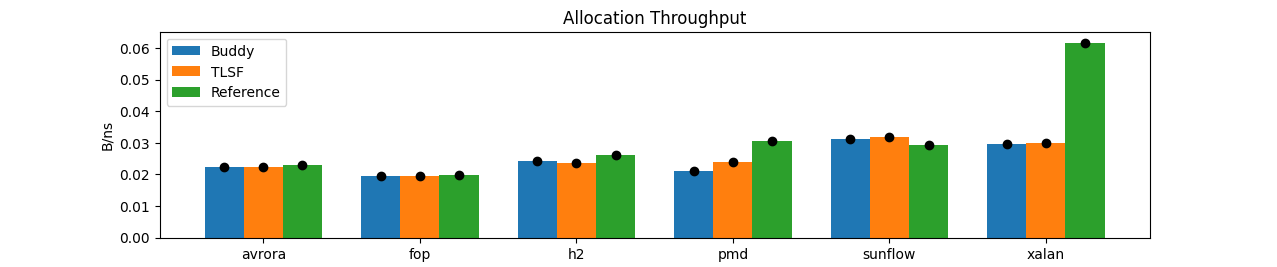
\includegraphics[width=0.6\textwidth]{figures/allocation_throughput.png}
\caption{Barplot showing the allocation throughput of the different allocation strategies when performing relocations.}
\label{fig:allocation-throughput}
\end{figure}

\subsubsection{Free List Initialization Throughput}

In order to measure the cost of searching for the free memory in the fragmented memory of a page, the initialization process of the free-list was introduced. Results shown in Figure~\ref{fig:free-list-initialization} show the throughput you get of initializing the free list. The numbers displayed show us that there is a significant cost to initializing the free list. Important to note here is that the difference in throughput between each of the benchmarks is because of the allocation patterns of the programs, and not a variatation in the performance of the machine running the program. 

\begin{figure}[H]
\centering
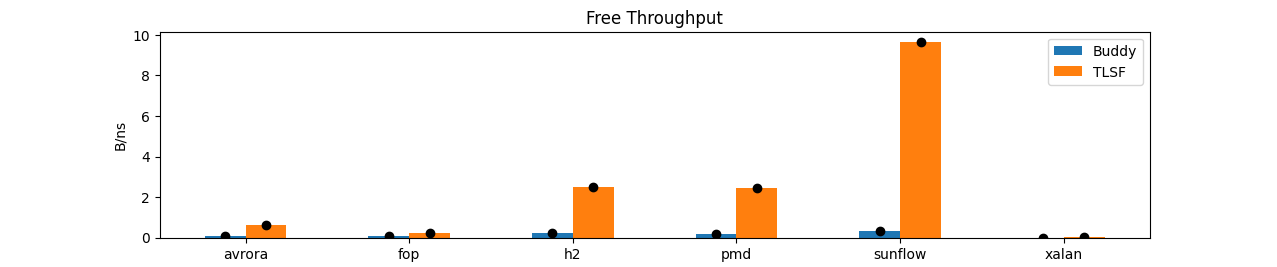
\includegraphics[width=0.6\textwidth]{figures/free_throughput.png}
\caption{Barplot displaying the througput of adding bytes of free memory to the allocator's free-list. The throuhgput is calculated as the amount of bytes found in the fragmented memory, divided by time it took to execute the initialization process.}
\label{fig:free-list-initialization}
\end{figure}

\subsubsection{Fragmentation}
The different allocators demonstrate a significant difference in their ability to makes use of the avaiable memory, displaying some huge variations in how much memory is able to be claimed before an allocation is too large to handle. This is evident from Figure~\ref*{fig:memory-fragmentation}. The plot shows different results for different benchmarking programs, but the TLSF allocator performs significantly better on all benchmarks.

%TODO kanske lägga in samma plot fast med maxreloc_2048 för att få niceigare värden :D 

\begin{figure}[H]
\centering
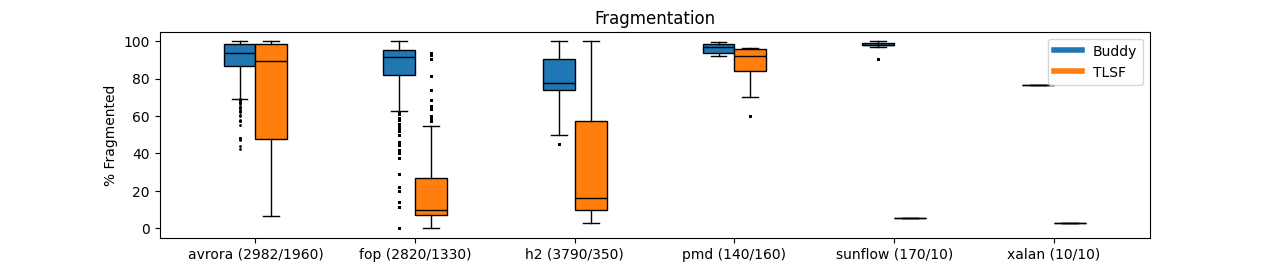
\includegraphics[width=0.6\textwidth]{figures/fl_fragmentation.png}
\caption{Boxplots for each benchmark, and different boxplots for the two implementations measured. Each measured data point is taken from the set of exhausted pages from a full run of the specified benchmark. The fragmentation is measured as the amount of used up bytes, divided by the total amount of bytes available. The numbers displayed by the benchmark name denotes the amount of data points measured for each implementation.}
\label{fig:memory-fragmentation}
\end{figure}

\subsection{Benchmark Performance}
This section evaluates the garbage collector's performance across various benchmarks, focusing on the Java program in its entirety while running with the new implementation of ZGC using free list allocators and comparing that to the reference version of ZGC that the new implementation is built upon.


\subsubsection{Relocation Duration}

Although overall execution time remains stable, there's a marginal increase in time that the garbage collector spends in the relocation phase. In Figure~\ref{fig:relocation-duration}, the relocation duration over multiple runs is shown. It is possible to see a slight upward trend in relocation time for the implementations using free-list relocations. 

\begin{figure}[H]
\centering
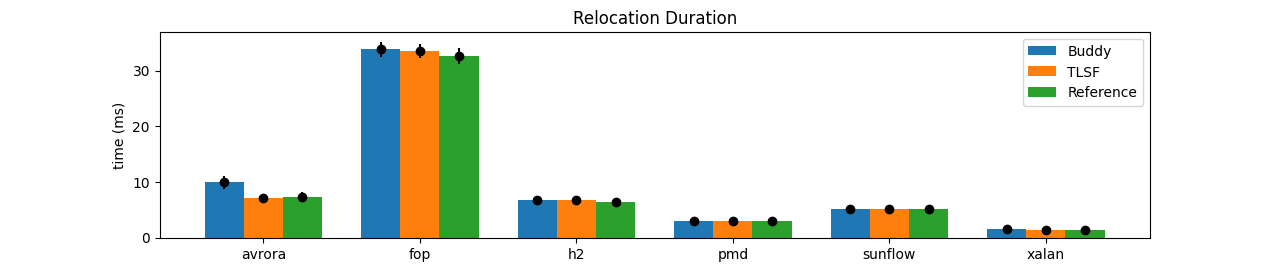
\includegraphics[width=1\textwidth]{figures/relocation.png}
\caption{Barplot showing the average duration that the garbage collector spent in the relocation phase, which is the phase where the reference version is only using bump pointer allocations, while the buddy allocator, and TLSF allocator are making use of a free-list allocation method, as well as resorting to bump pointers when needed.}
\label{fig:relocation-duration}
\end{figure}

\subsubsection{Relocation Set Selection Duration}

This metric shows the time it takes for the garbage collector to select which pages are going to be used for relocation, which is the phase impacted by the initialization of free list memory. In Figure~\ref{fig:set-selection}, a barplot is showing the average time that the different implementations spend in the relocation set selection phase of the garbage collection cycle.

\begin{figure}[H]
\centering
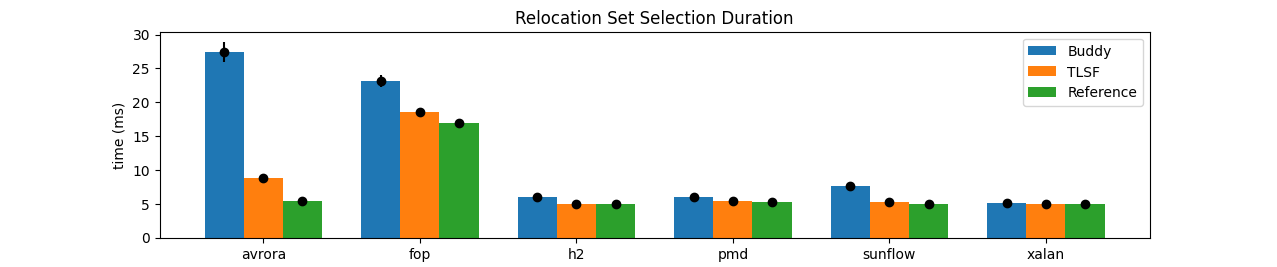
\includegraphics[width=1\textwidth]{figures/set_selection.png}
\caption{Barplot showing the averelocation set Selection Duration Comparison}
\label{fig:set-selection}
\end{figure}


\subsubsection{Throughput}
Through repeated benchmark executions, the execution time remains largely consistent across all implementations, with overlapping confidence intervals. In Figure~\ref{fig:execution-time}, the exeuction times are displayed from running the six different benchmarks for 250 iterations each, comparing the three different implementations.

\begin{figure}[H]
  \centering
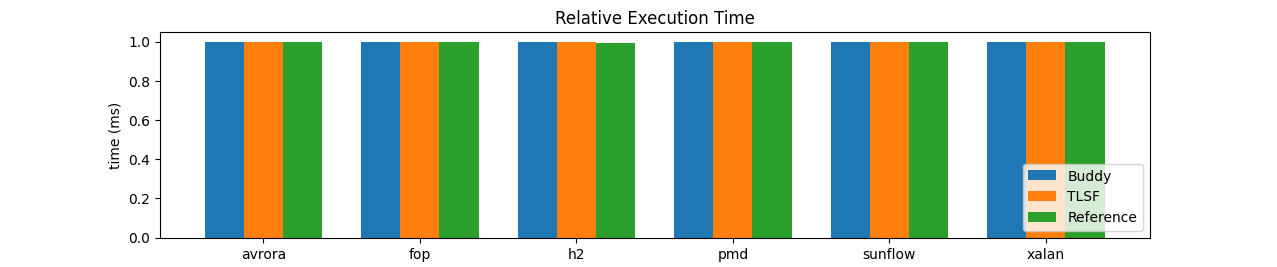
\includegraphics[width=1\textwidth]{figures/execution_time.png}
\caption{Throughput Comparison Across Benchmarks}
\label{fig:exeuction-time}
\end{figure}
